\documentclass{article}

%% doc settings
\hyphenchar\font=-1 % suppress hyphenation
\setlength\parindent{0pt} % suppress indentation
\usepackage[margin=1.25truein]{geometry} % set page margins

%% libraries
\usepackage{listings}
\usepackage{fancyhdr}
\usepackage{lastpage}
\usepackage{url}
\usepackage{xcolor}
\usepackage{hyperref}
\usepackage{amssymb}
\usepackage{amsthm}
\usepackage{amsmath}
\usepackage{natbib}
\usepackage{tikz}
\usepackage{pgfplots}
\usepackage{textcomp}
\usepackage{subcaption}
\usetikzlibrary{shapes, arrows}

%% link viz
\hypersetup{
    colorlinks = true,
    linkcolor = red,
    urlcolor = red,
    citecolor = black
}

%% code colors 
\definecolor{codegreen}{rgb}{0,0.6,0}
\definecolor{codegray}{rgb}{0.5,0.5,0.5}
\definecolor{codepurple}{rgb}{0.58,0,0.82}
\definecolor{backcolour}{rgb}{0.95,0.95,0.92}

\lstdefinestyle{mystyle}{
    backgroundcolor=\color{backcolour},   
    commentstyle=\color{codegreen},
    keywordstyle=\color{magenta},
    numberstyle=\tiny\color{codegray},
    stringstyle=\color{codepurple},
    basicstyle=\ttfamily\footnotesize,
    breakatwhitespace=false,         
    breaklines=true,                 
    captionpos=b,                    
    keepspaces=true,                 
    numbers=left,                    
    numbersep=5pt,                  
    showspaces=false,                
    showstringspaces=false,
    showtabs=false,                  
    tabsize=2
}

\lstset{style=mystyle}

%% page nums
\pagestyle{fancy}
\fancyhf{}
\fancyfoot[C]{Pg. \thepage \space of \pageref*{LastPage}}
\renewcommand{\headrulewidth}{0pt}

%% begin doc
\begin{document}
\title{SYSEN 6000: Foundations of Complex Systems\\~\\
    \Large Non-Linear Dynamics \& Chaos
}
\author{
    Nick Kunz [NetID: \url{nhk37}] \hyperlink{nhk37@cornell.edu}{nhk37@cornell.edu}}
\date{October 21, 2022}
\maketitle
\thispagestyle{fancy}

%% body doc
\section*{SIR Model}
The Susceptible, Infected, and Removed (SIR) Model is commonly applied in epidemiology to model disease transmission. It can be expressed as:

    \begin{equation}
    \begin{split}
        S' & = -\alpha \cdot SI \\
        I' & = \alpha \cdot SI - \beta I \\
        R' & = \beta I
    \end{split}
    \end{equation}

When $n=800$, $\alpha = 2.2 \cdot 10^{-3}$, and $\beta = 0.4$, the phase plane solution can be illustrated as:

    \begin{figure}[h]
        \centering
        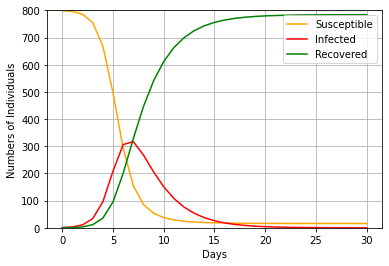
\includegraphics[width=0.6\textwidth]{800.png}
        \caption{SIR Model General Application}
        \label{fig:sir_800}
    \end{figure}
    
Computing $\rho$, when $\rho = \beta / \alpha$, we see that:
    \begin{equation}
    \begin{split}
        \rho 
            & = 0.4 / 2.2 \cdot 10^{-3} \\
            & = 181.82
    \end{split}
    \end{equation}

\newpage
In the English Boarding School case of 1978, when $n = 1,000$, the phase plane solution can be illustrated as:

    \begin{figure}[h]
        \centering
        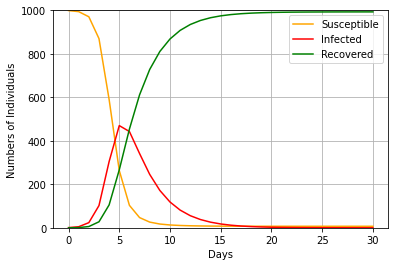
\includegraphics[width=0.6\textwidth]{1000.png}
        \caption{SIR Model English Boarding School House of 1978}
        \label{fig:sir_1000}
    \end{figure}

The SIR Model could exhibit chaos like below by changing variables in higher dimensions \cite{dynamics} \cite{subharm}.

\section*{Chaos Theory}

Considering the Rossler model for chemical reactions, the dynamics can be represented by dimensions $X, Y, Z$, which have quadratic non-linearity similar to the SIR model and can be expressed as:
    \begin{equation}
    \begin{split}
        X' & = -(Y + Z) \\
        Y' & = X + \alpha Y \\
        Z' & = \beta + (X - c) Z
    \end{split}
    \end{equation}

Integrating through the first two period doubling of the Rossler model can be illustrated as:
    
    \begin{figure}[h]
        \centering
        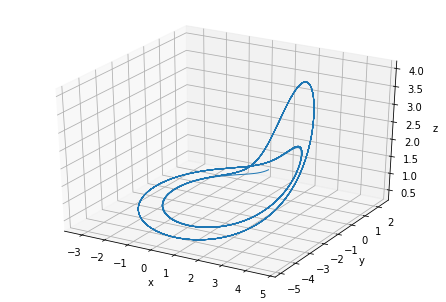
\includegraphics[width=0.6\textwidth]{rossler.png}
        \caption{Rossler's Model Phase Space \cite{moon}}
        \label{fig:rossler}
    \end{figure}

\section*{Fractal Geometry}
The \textit{``Sierpinksi Carpet''} begins with a square and is divided into nine sub-squares. The central square is removed and repeated for each of the remaining sub-squares.\\


It's dimension can be expressed simply as:
    \begin{equation}
    \begin{split}
        - \lim\limits_{m \to \infty} \frac{\log N(\epsilon_m)}{\log \epsilon_m} = - \lim\limits_{m \to \infty} = \frac{m \log 8}{m \log 3} = \frac{\log 8}{\log 3}
    \end{split}
    \end{equation}\\

and can be illustrated as such:

    \begin{center}
        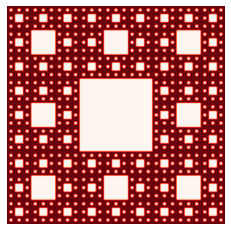
\includegraphics[width=0.55\textwidth]{carpet.png}
    \end{center}


%% ref sec
\newpage
\bibliographystyle{ieeetr}
\bibliography{ref.bib}

\newpage
\section*{Appendix}
\begin{enumerate}
    \item SIR Model
    \begin{lstlisting}[language=Python, title=Python 3: SIR Model for English Boarding School House of 1978]
## libraries
import numpy as np
import pandas as pd
import matplotlib.pyplot as plt
from scipy.integrate import odeint

## params
n = 1000
alpha = 0.002
beta = 0.4

## init
i = 1
s = n - i
r = 0
t_max = 30
t = np.linspace(0, t_max, t_max + 1)

## sir model
def sir_der(y, t, alpha, beta):

    s, i, r  = y
    ds_dt = -alpha * s * i
    di_dt = alpha * s * i - beta * i
    dr_dt = beta * i

    return [ds_dt, di_dt, dr_dt]

## derive
y = s, i, r
res = odeint(sir_der, y, t, args = (alpha, beta))
s, i, r = res.T

## plot
plt.figure()
plt.grid()
plt.plot(t, s, 'orange', label = 'Susceptible')
plt.plot(t, i, 'r', label = 'Infected')
plt.plot(t, r, 'green', label = 'Recovered')
plt.xlabel('Days')
plt.ylabel('Numbers of Individuals')
plt.ylim([0, n])
plt.legend()
plt.show()\end{lstlisting}

\newpage
    \item Rossler Model 
    \begin{lstlisting}[language=Python, title=Python 3: Rossler Model for Chemical Reactions]
## libraries
import numpy as np
import matplotlib.pyplot as plt
from mpl_toolkits.mplot3d import Axes3D

## dynamics
def rossler(x, y, z, a, b, c):

    x_dot = -(y + z)
    y_dot = x + a * y
    z_dot = b + (x - c) * z

    return x_dot, y_dot, z_dot

## differ rate
def rossler_differ(step, dt):

    xs = np.empty((step + 1,))
    ys = np.empty((step + 1,))
    zs = np.empty((step + 1,))

    xs[0], ys[0], zs[0] = (1.0, 1.0, 1.0)

    for i in range(0, step):
        x_dot, y_dot, z_dot = rossler(
            x = xs[i], 
            y = ys[i], 
            z = zs[i],
            a = 0.35,
            b = 2.00,
            c = 4.00
        )

        xs[i+1] = xs[i] + (x_dot * dt)
        ys[i+1] = ys[i] + (y_dot * dt)
        zs[i+1] = zs[i] + (z_dot * dt)

    return xs, ys, zs

## comp traj
xs, ys, zs = rossler_differ(
    step = 100000,
    dt = 0.001
)

## plot
fig = plt.figure()
ax = Axes3D(fig)
ax.plot(xs, ys, zs, lw = 1)
ax.set_xlabel('x')
ax.set_ylabel('y')
ax.set_zlabel('z')
plt.show()\end{lstlisting}

\newpage
    \item Fractal Geometry
    \begin{lstlisting}[language=Python, title=Python 3: Fractal Geometry for Sierpenski Carpet]
## libraries
import numpy as np
import matplotlib.pyplot as plt

## make square
def square(x, y, len, img):
    for i in range(x, x + len):
        for j in range(y, y + len):
            img[i, j] = 0

    return img

# ## sierpinski carpet
def sierp_carpet(lev = 4):

    len = 3 ** lev

    img_sq = np.full(
        shape = (len, len),
        fill_value = 1
    )

    len_i = lev + 1
    for i in range(1, len_i):
        len_sq = int(
            len / (3**i)
        )

        len_j = 3 ** i
        for j in range(0, len_j, 3):
            x_j = int(
                (j + 1) * len_sq
            )
            
            len_k = 3 ** i
            for k in range(0, len_k, 3):
                y_k = int(
                    (k + 1) * len_sq
                )

                img_sq = square(
                    x = x_j, 
                    y = y_k, 
                    len = len_sq, 
                    img = img_sq
                )

    return img_sq

## make carpet
carpet = sierp_carpet()

## plot
plt.axis('off')
plt.imshow(carpet, cmap = 'Reds')
plt.show()\end{lstlisting}

\end{enumerate}


\end{document}